\chapter{Introduction}
\label{c:intro}

% 動機
\section{Motivation}
\label{section:motivation}

\subsection{Previus Solution}
%\label{subsection:previus-solution}
add previus work here.



\section{Related Works}
\label{section:related-work}
% add something here

\section{Goal}
\label{section:goal}
Design a system that is both cost efficient and time efficient. Can handle 

\section{Divide and Conquer}
\subsection{Definition}
\label{section:divide-and-conquer}

Fig.~\ref{fig:DnC} shows the concepts of \emph{divide and conquer} (D\&C). D\&C is an algorithm design paradigm that breaks a complex problem into a couple of relatively simple subproblems, to \emph{divide}, then solves them respectively, to \emph{conquer}. Before conquering, the problem will be divided recursively until it is simple enough to be processed. Finally, the solutions to the subproblems will be merged as those to the original problem.

\begin{figure}[!htb]
    \centering
    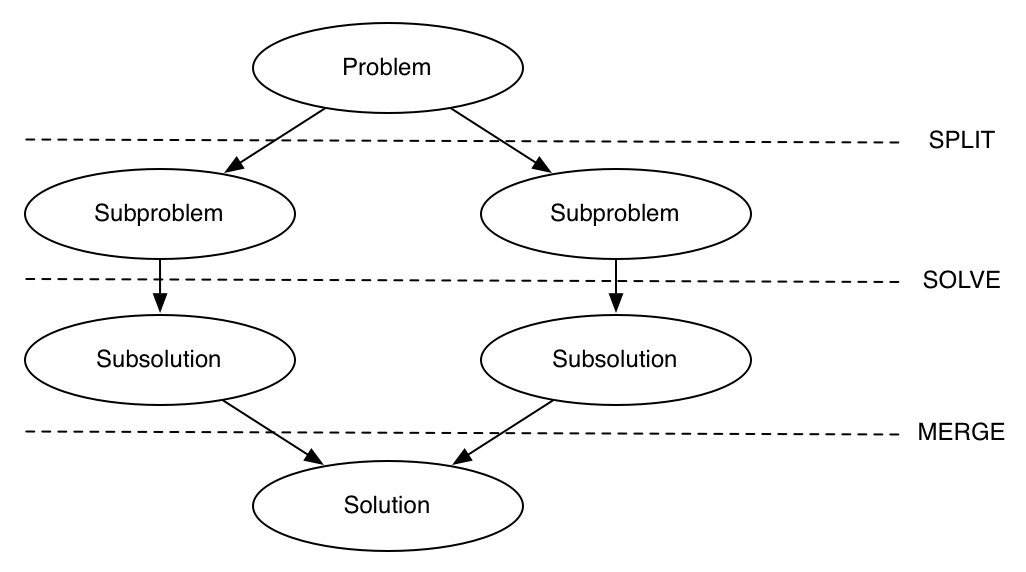
\includegraphics[width=\textwidth]{figsrc/DnC.png}
    \caption{A diagram showing how divide and conquer works.\label{fig:DnC}}
\end{figure}

% 論文貢獻
\subsection{Main Contribution of This Dissertation}
\label{subsec:advantages}

\subsubsection{Reducing the Difficulty of Problems}

Due to characteristics of D\&C, all problems that can be accurately split are expected to be solved. For this dissertation, particularly, if the function detecting staves is reliable, then we can analyze arbitrarily complicated scores.

\subsubsection{Independence of Subproblems}

Typically, a score contains something useless for recognition such as the metadata of the song, lyrics, and even printed defects. By partitioning the original images into subimages where each contains only one staff, the amount of noisy information can be reduced and interference between staves is eliminated. Therefore, the detection tasks are independent between different staves.

\subsubsection{Parallelism}

Nowadays, a processor usually has multiple cores, and lots of computational tasks are implemented to be executed with parallel programs. In D\&C algorithm, the functions solving split subproblems are identically designed. With high independence and similar operations between subproblems, it is a good strategy to process them simultaneously. In other word, the original problem is suitable to be solved with \emph{SIMD (Single-Instruction-Multiple-Data)} parallel programs.
